%
% introduction.tex
%
% Copyright (C) 2023 UFSC.
%
% DOCUMENTATION-TEMPLATE
%
% This work is licensed under the Creative Commons Attribution-ShareAlike 4.0
% International License. To view a copy of this license,
% visit http://creativecommons.org/licenses/by-sa/4.0/.
%
% aluno
% 1 - risc-v: intructions architectures. nao precisa colocar como as instruções são executadas (pipeline). colocar os registradores. colocar imagens mais simples da arquitetura do risc-v. diferença de microprocessador e microntrolador.
% 2 - mostra a cpu  e os perifericos, so que nao na primeira aula. na primeira aula so CPU e os registradores. o que é o mapeamento de memória? o que acontece nos registradores? 
% 2-3 agrupar conforme as aulas do 8051.
% 4 - aprensentar no inicio do documento
% 5 - deixa onde estar

% professor
% 1 - pipeline, risc-v instructions
% 3.2 - livro do técnico

\chapter{RISC-V} \label{ch:chapter_riscv_prof}

Welcome to \autoref{ch:chapter_riscv_prof}, dedicated to analyzing and explaining the RISC-V architecture, explaining each block and the operation of the pipeline, as well as a brief look at the instruction set.

The following sections will provide a comprehensive overview of the fundamental components of a RISC-V architecture processor.

\autoref{sec:section_riscv_prof.1}:
    In this subsection, we will cover the basic topics about RISC-V architecture, comprising the combinational elements, the sequential elements, the clocking methodology, instruction lookup, instruction types, and the composition of the elements.
    
\autoref{sec:section_riscv_prof.2}:
In this subsection, we will talk about the RISC-V architecture, understanding its aspects of operation such as an overview of the CPU, multiplexers, control, datapath, the instruction types, ALU control, central control unit and pipeline including hazards.

\autoref{sec:section_riscv_prof.3}:
Finally, in this section we will cover about the instructions, understanding their operation with assembly.

    \section{RISC-V Basics} \label{sec:section_riscv_prof.1}
    
    In RISC-V the information is encoded in binary, where low voltage represents 0 and high voltage represents 1. Each bit of information is typically transmitted over a single wire, with multiple bits forming multi-bit data transmitted over multi-wire buses.

        \subsection{Combinational Elements} 
        
        Combinational elements operate on data by performing specific operations or transformations. These elements take input signals and produce output signals based on a defined logic function. The output is solely determined by the current input values and does not depend on any previous state or history.
        
        \subsection{Sequential Elements}
        
         Sequential elements or state elements, are used to store information and introduce memory into the system. They maintain a state that can change over time based on the inputs and the current state. Sequential elements, such as flip-flops or registers, store and remember information, allowing for sequential and memory-dependent operations.
        
        \subsection{Clocking Methodology}
        
        The clocking methodology used in RISC-V processors follows a synchronous clocking approach. In RISC-V, a central clock signal is generated and distributed to all the components within the processor. The clock signal acts as a reference for the timing of instructions execution and synchronization of various operations.
        
        \subsection{Instruction Fetch}
        
        Instruction Fetch, also known as the fetch stage, is a step in the execution cycle of a RISC-V processor. In this stage, the processor retrieves the next instruction to be executed from memory.
        
        \subsection{R-Format Instructions}
        
        R-Format instructions in the RISC-V architecture are instructions that operate on registers. They have a fixed 32-bit structure with specific fields for the operation type, source and destination registers, and additional function bits. These instructions perform arithmetic, logical, and data manipulation operations by using the values in the source registers and storing the result in the destination register. They provide flexibility and efficiency by allowing direct register-to-register operations, making them essential for data processing in the RISC-V architecture.
        
        \subsection{Load/Store Instructions}
        
        Load/Store instructions in the RISC-V architecture facilitate the transfer of data between registers and memory. Load instructions retrieve data from memory and store it in a register, while store instructions take data from a register and store it in memory. These instructions are essential for data manipulation and memory access in RISC-V programs, enabling efficient reading from and writing to memory locations.
        
        \subsection{Branch Instructions}
        
        Branch instructions in the RISC-V architecture are used for conditional branching, allowing programs to alter the flow of execution based on certain conditions. These instructions compare values in registers and determine whether to branch to a different instruction or continue sequentially. Branch instructions are essential for implementing control flow, such as loops and conditional statements, in RISC-V programs. They enable program execution to make decisions and follow different paths based on the evaluated conditions, enhancing the flexibility and versatility of the architecture.
        
        \subsection{Composing the Elements}
        
        Composing the elements in the RISC-V architecture involves combining different components to create a functional system. This includes integrating the CPU core, memory subsystem, input/output interfaces, and other peripherals. The elements are interconnected through buses or interconnects, enabling communication and data transfer between them. The composition of these elements requires careful design and consideration to ensure proper functionality and performance of the RISC-V system as a whole.

    \section{RISC-V Architecture} \label{sec:section_riscv_prof.2}
    
    The RISC-V architecture will be studied in the following subsections. The idea is to start with a simplified diagram of the processor and gradually add architecture blocks.

        \subsection{CPU Overview}
        
        A RISC-V CPU (Central Processing Unit) is the central component of a computer system that executes instructions based on the RISC-V instruction set architecture. The CPU fetches instructions from memory using the Program Counter (PC) and decodes them to determine the operation and involved operands. Next, the CPU executes the instruction by performing the arithmetic, logical, memory access, or control flow operations specified by the instruction and updates registers or memory \cite{patterson}.
        
                \begin{figure}[!h]
        	    \centering
        	    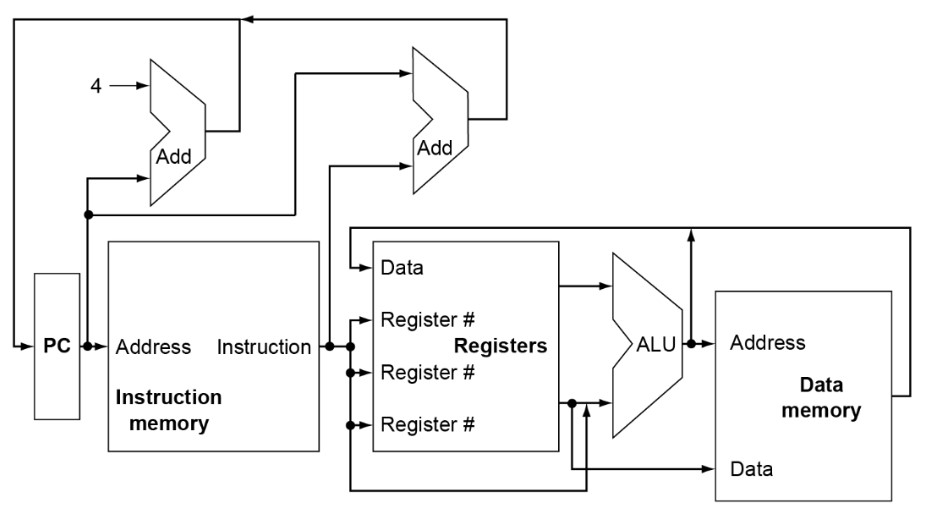
\includegraphics[width= 0.7
        	    \textwidth]{figures/riscv/risc_1.jpg}
                    \caption{\label{risc_1} CPU Overview Diagram}
                \end{figure}
        
        Figure \ref{risc_1} show an overview of the key components of the RISC-V CPU, where ``PC'' is the program counter, an 32-bit or 64-bit register; the ``Add'' are adders; ``Instruction Memory'' refers to the component of the processor that stores and provides the instructions to be executed by the processor; ``Registers'' are small storage units within the processor that hold data and instructions during program execution. They are used for fast and efficient data manipulation, storing intermediate values, and holding the results of computations; ``ALU'' is the arithmetic logic unit; and ``Data memory'' is the part of the processor that stores and retrieves data during program execution. It provides a space for reading and writing data, allowing the processor to access and manipulate variables, arrays, and other data structures required by the program. 
        
        
        \subsection{Multiplexers}
        
        Multiplexers (MUX), are critical components used for selecting one of several inputs to be passed as the output. This components play a significant role in data routing and control signal selection within the CPU, for example, in the Figure \ref{risc_1a} it is necessary to put an MUX in each red circle, as it is not possible to simply join the wires.
        
                \begin{figure}[!t]
        	    \centering
        	    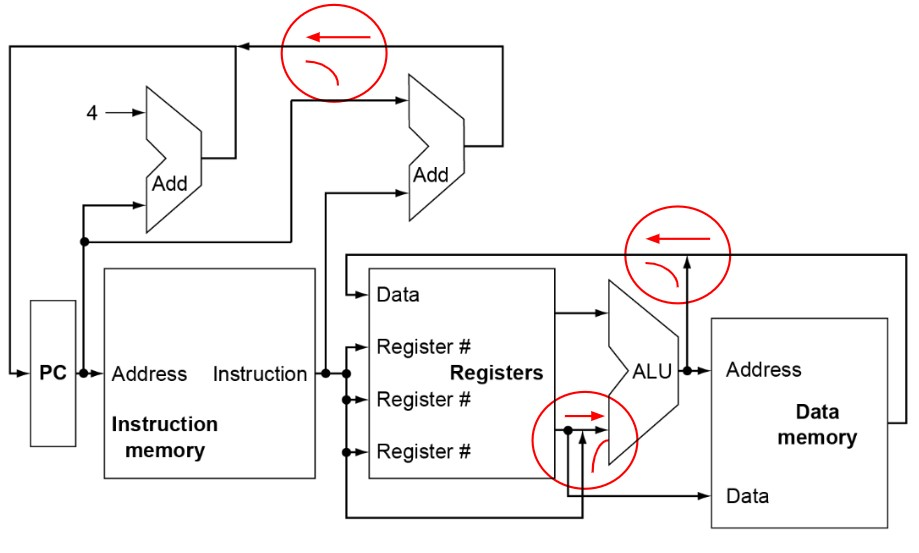
\includegraphics[width= 0.7
        	    \textwidth]{figures/riscv/risc_1a.jpg}
                    \caption{\label{risc_1a} Diagram showing where multiplexers are needed}
                \end{figure}
        
        \subsection{Control}
        
        Control in RISC-V architecture is responsible for decoding instructions, generating the necessary control signals, and coordinating the execution of operations within the CPU. The control unit determines which components should be activated or deactivated, such as the ALU, registers, and multiplexers, to perform the operations specified by the instructions.
        
                \begin{figure}[!h]
        	    \centering
        	    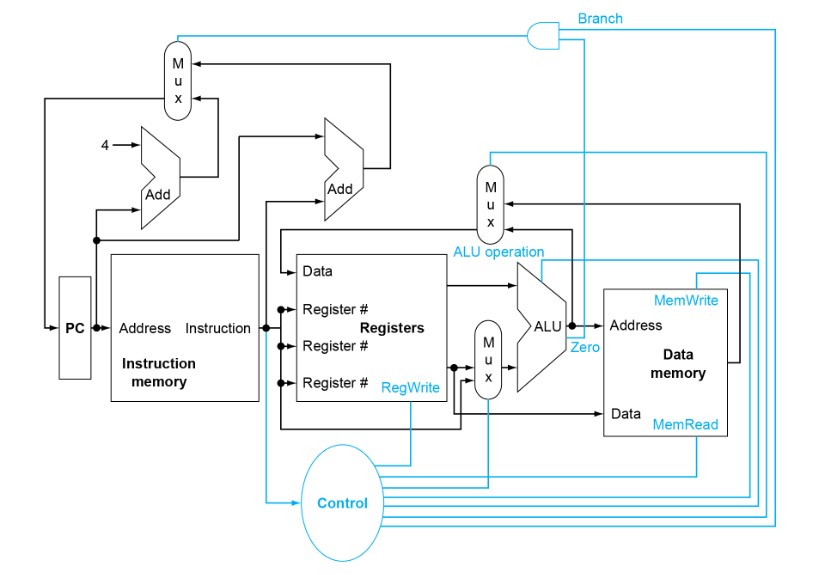
\includegraphics[width= 0.8
        	    \textwidth]{figures/riscv/risc_2.jpg}
                    \caption{\label{risc_2} Diagram with added control signals}
                \end{figure}
                
        Figure \ref{risc_2} shows the control unit and its connections in blue. At this first moment, the control is only used in ``RegWrite'', indicating if the result of an instruction must be written back in a register; ``MemRead'' and ``MemWrite'' to indicate whether a memory read or write operation should be performed; ``Branch'' used for implementing conditional branching or jump operations. In control, the ``ALUOperation'' signal can have different values, each corresponding to a specific operation that the ALU should perform. Some common examples of operations controlled by ``ALUOp'' include addition, subtraction, logical operations (AND, OR, XOR), bit shifting, and comparisons. Finally, the ``Zero'' control signal refers to a flag or signal that indicates whether the result of an operation performed by the ALU is equal to zero. This flag is used to make conditional decisions based on the result of a previous operation.

        \subsection{Full Datapath}

            In Figure \ref{risc_4} you can see the full RISC-V Diagram, where all the blocks that have been added sequentially are present. 
            
                    \begin{figure}[!h]
            	    \centering
            	    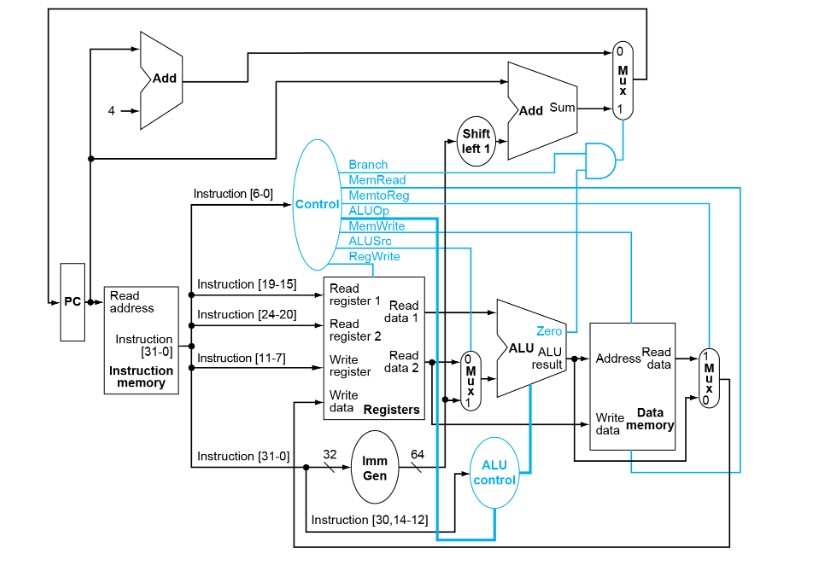
\includegraphics[width= 1
            	    \textwidth]{figures/riscv/risc_4.jpg}
                        \caption{\label{risc_4} RISC-V Full Datapath}
                    \end{figure}
            In the diagram, the specific bits of an instruction are routed to the different control blocks and functional units of the processor as follows:
    
            \begin{itemize}
            \item Bits [6-0] are connected to the control block. These bits are used to determine the specific operation that the instruction will perform.
            \item Bits [19-15] are used to select the read register 1. These bits indicate which register will be read to provide one of the operands for the operation.
    
            \item Bits [24-20] are used to select the read register 2. These bits indicate which register will be read to provide the second operand for the operation.
    
            \item Bits [11-7] are used to select the write register. These bits indicate in which register the result of the operation will be stored.
    
            \item Bits [31-0] are directed to the ``Imm Gen'' (Immediate Generation) block. These bits are used to generate the immediate value required by the instruction.
    
            \item Bits [30, 14-12] are used to control the control block of the Arithmetic Logic Unit (ALU). These bits determine the specific operation that the ALU will perform.
            \end{itemize}
        
        \subsection{R-Type/Load/Store Datapath}

            \begin{figure}[!h]
            \centering
            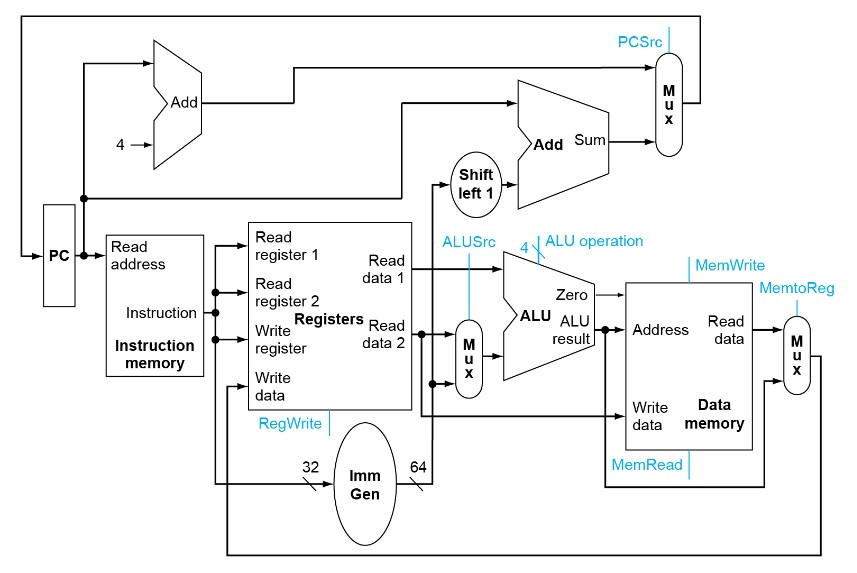
\includegraphics[width = 0.8
            \textwidth]{figures/riscv/risc_3.jpg}
                \caption{\label{risc_3} Diagram with added R-Type/Load/Store signals}
            \end{figure}

            At this time the R-Type, Load and Store instructions in the Diagram are added (Figure \ref{risc_3}). In the representation, ``ALU Src'' (ALU Source) is a control signal that determines the input data source to the Arithmetic Logic Unit (ALU) during the execution of an instruction. Specifically, the ALU Src signal determines whether the input value to the ALU will come from a register or an immediate value; ``PC Src'' (PC Source) in RISC-V is a control signal that determines the data source used to update the value of the PC during the instruction fetch cycle; ``MemToReg'' (Memory to Register) is a control signal in the RISC-V architecture that determines whether the data loaded from memory should be written back to a register in an instruction execution cycle; and ``Imm Gen'' (Immediate Generation) is a unit responsible for generating the immediate value used in instructions that involve operations with constant values embedded within the instruction itself.
    
            Shown below are three examples of the processor and Datapath with Control parts used in three different types of R-Type, Load, and BEQ instructions. 
        
            \subsubsection{R-Type Instruction}
        
                \begin{figure}[!h]
                \centering
                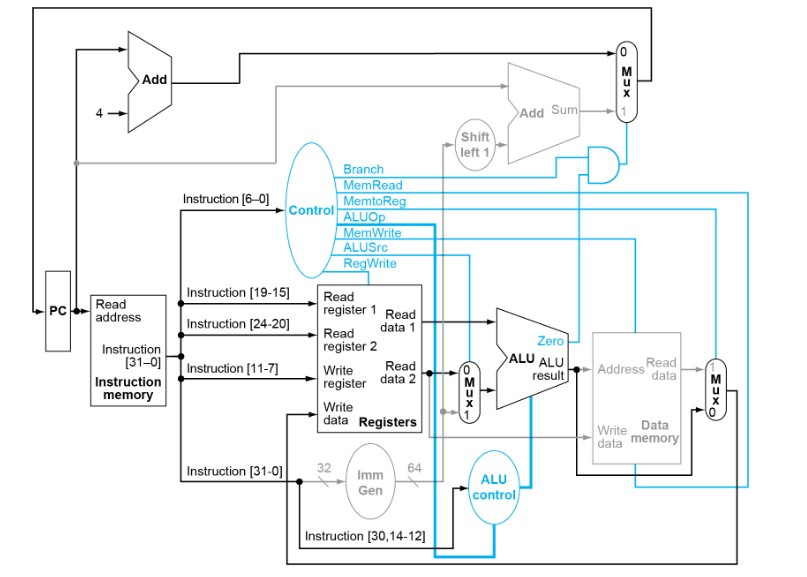
\includegraphics[width= 0.8
                \textwidth]{figures/riscv/risc_R-type.jpg}
                    \caption{\label{risc_R-type} RISC-V R-Type}
                \end{figure}
                
                Figure \ref{risc_R-type} shows the processor diagram executing an R-Type instruction. The gray parts represent the parts of the processor that are not being used and the blue parts represent the control part. In this instruction, the Imm Gem blocks are not used and values are not written to the memory, as well as the PC receives an increase of four units.  In this format, the instruction has three registers as operands and a destination register where the result will be stored. The operations supported by the R-type format include addition, subtraction, multiplication, division, logical operations (AND, OR, XOR), and shifting. The R-type instruction is widely used to perform calculations and data manipulations within the RISC-V processor.
            
            \subsubsection{Load Instruction}

                \begin{figure}[!h]
                \centering
                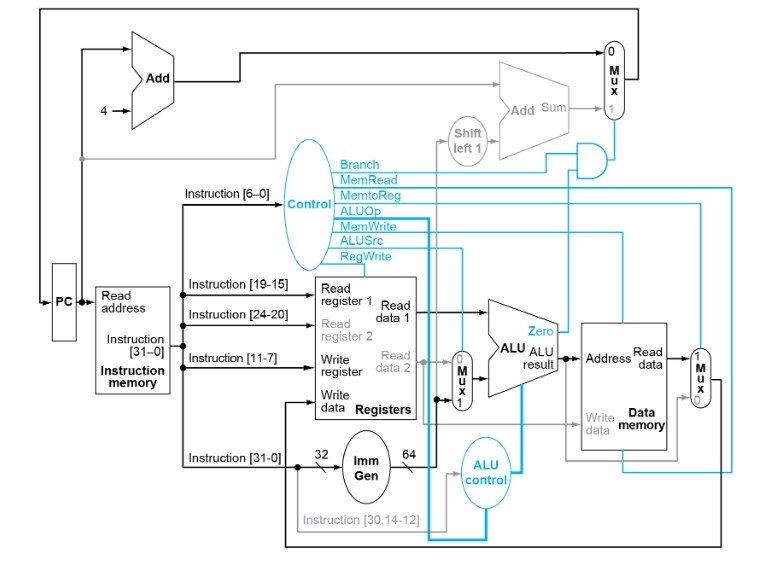
\includegraphics[width= 0.8
                \textwidth]{figures/riscv/risc_L-type.jpg}
                    \caption{\label{risc_L-type} RISC-V Load Instruction}
                \end{figure}

                On the other hand, Figure \ref{risc_L-type} shows a Load instruction being executed. Note that in this instruction only Imm Gen is used, and memory values are read. The Load instruction in RISC-V is used to fetch a value from memory and load it into a specific register. It allows the processor to access and use data stored in memory. The Load instruction typically requires specifying the memory address from where the data should be fetched and the destination register where the data will be stored. It is an essential instruction for reading data from memory and is used in various data processing operations, such as accessing array elements, reading variables, or retrieving data from external devices.
            
            \subsubsection{BEQ Instruction}

                \begin{figure}[!h]
                \centering
                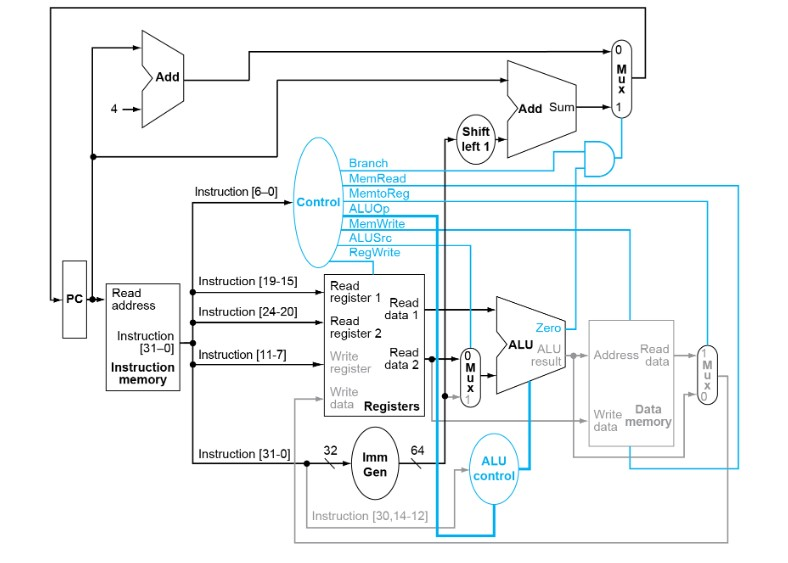
\includegraphics[width= 0.8
                \textwidth]{figures/riscv/risc_BEQ-type.jpg}
                    \caption{\label{risc_BEQ-type} RISC-V BEQ Instruction}
                \end{figure}

                In the case of Figure \ref{risc_BEQ-type} a BEQ (Branch if Equal) instruction is presented. This type of instruction does not access memory, is a conditional branch instruction that checks if two registers are equal and performs a branch to a specified address if the condition is true. It is used to control the flow of program execution based on equality comparisons between register values. The BEQ instruction is used to implement conditional control structures such as loops and decision structures, allowing the program to take different execution paths based on the specified conditions.                

       \subsection{ALU Control}

            The ALU (Arithmetic Logic Unit) control in RISC-V is responsible for determining the operation to be performed by the ALU based on the instruction. It decodes the relevant fields of the instruction and generates control signals to configure the ALU accordingly. This enables the ALU to execute arithmetic, logical, and bitwise operations as specified, contributing to data processing in the RISC-V processor.
        
        
       \subsection{The Main Control Unit}

            The Main Control Unit controls the data flow between the memory, instruction register, data register, ALU, and other elements of the processor. It ensures that instructions are executed correctly by coordinating memory access, instruction fetching and decoding, and data manipulation.
            
            Moreover, the Main Control Unit implements the control logic that determines the next state of the processor based on the current instruction. This includes selecting the next instruction address, controlling registers, and generating the appropriate control signals for each component of the processor.
            
        \subsection{RISC-V Pipeline}
            
            The RISC-V architecture supports a five-stage pipeline known as the RISC-V pipeline. The five stages of the pipeline are:
            \begin{enumerate}
            \item Instruction Fetch (IF): In this stage, the processor fetches the instruction from memory. The program counter (PC) is used to fetch the instruction from the memory address pointed to by the PC.
            \item Instruction Decode (ID): In this stage, the fetched instruction is decoded, and the necessary control signals and register operands are prepared for the subsequent stages. The register operands are read from the register file, and immediate values are sign-extended if needed.
            \item Execute (EX): In this stage, the ALU (Arithmetic Logic Unit) performs the arithmetic or logical operation specified by the instruction. This stage also handles branch and jump instructions, where the target address is computed.
            \item Memory Access (MEM): In this stage, memory operations such as load and store are performed. For load instructions, the memory is accessed to retrieve the required data, while store instructions write data from a register to the memory.
            \item Write Back (WB): In this final stage, the results of the executed instruction are written back to the register file. This includes the result of ALU operations or the data loaded from memory.
            
            \end{enumerate}
            
            Implementing a pipeline in RISC-V can significantly increase processor performance. Similar to the example in Figure \ref{pipe2}, pipeline divides instruction processing into sequential stages, allowing multiple instructions to be executed in parallel and speeding up the processing rate.
            
            \begin{figure}[!h]
            \centering
            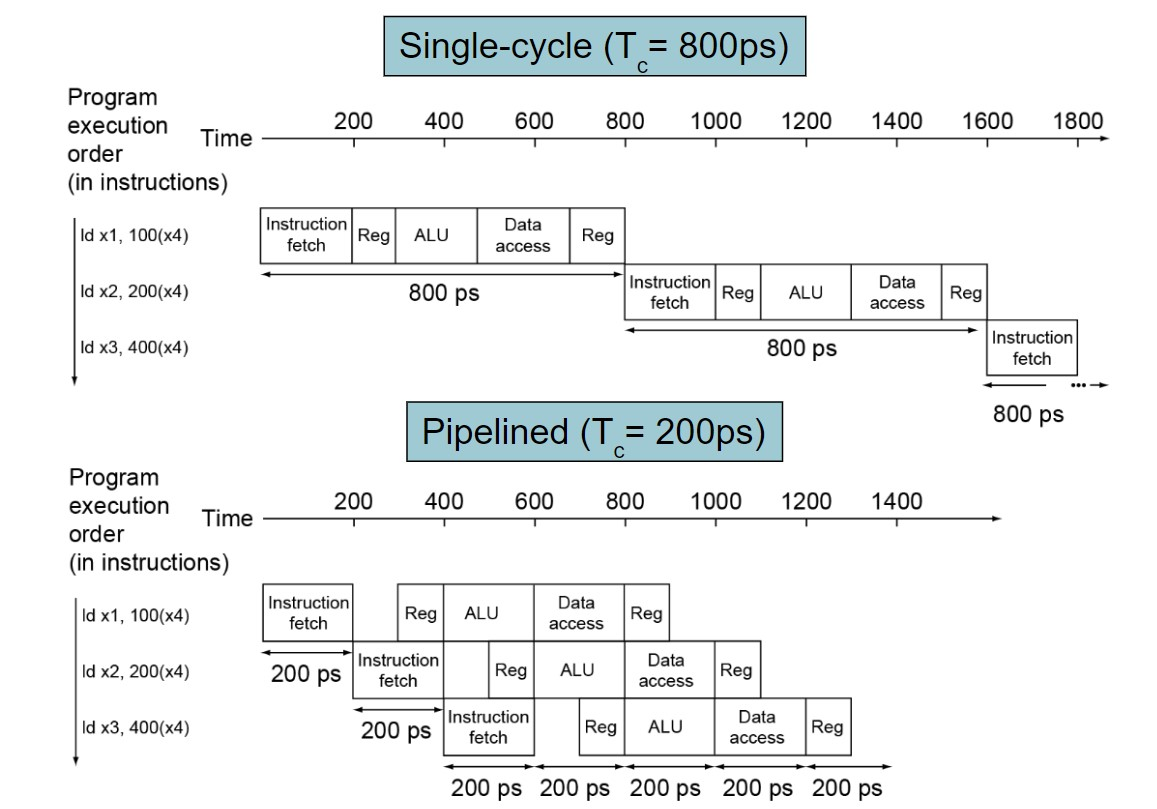
\includegraphics[width=0.8\textwidth]{figures/riscv/pipe2.jpg}
                \caption{\label{pipe2} Pipeline performance representation }
            \end{figure}

    
            \subsubsection{Hazards}

                Hazards are situations where the correct and efficient execution of instructions is hindered due to data dependencies or the sequential nature of instructions. Hazards can result in pipeline delays, reducing the performance of the processor. There are three main types of hazards in RISC-V:

                \begin{itemize}

                \item Data Hazard: Occurs when an instruction depends on a result produced by a previous instruction that has not yet completed. This can occur in cases of reading a value that has not been written yet or writing to a register before its value is read by subsequent instructions.

                \item Control Hazard: Occurs when a conditional branch instruction alters the normal flow of program execution. This can result in uncertainty about which instruction will be executed next, causing delays in instruction fetch and forwarding of subsequent instructions.
                
                \item Structural Hazard: Occurs when there is a conflict in physical resources of the processor, such as functional units, memory, or registers. This can occur when two instructions need to access the same resource simultaneously, resulting in delays and potentially requiring instruction reordering.
                \end{itemize}
                
                To deal with hazards in RISC-V, various techniques can be applied, such as data forwarding, instruction scheduling, branch prediction, and the use of buffers to avoid structural conflicts.

    \section{RISC-V Instructions} \label{sec:section_riscv_prof.3}

        \subsection{Arithmetic instructions use register
        operands}
        
            In RISC-V, there are 32 general-purpose registers, labeled from x0 to x31. These registers are 64 bits wide and can hold data or addresses.
            
            Here is a brief overview of the common uses and conventions for some of the registers in RISC-V:
            
            x0 (zero register): This register is hardwired to the constant value zero and cannot be modified. It is often used for special purposes such as encoding a constant zero value or serving as a destination for instructions that discard their results.
            
            x1 (ra, return address): This register is typically used to store the return address when executing function calls. It is usually automatically managed by the function calling convention.
            
            x2 to x7 (a0 to a7, argument registers): These registers are commonly used to pass function arguments. The first few arguments to a function are typically placed in these registers according to the function calling convention.
            
            x8 (t0 to t2, temporary registers): These registers are often used as temporary storage during computations within a function. They are not required to be preserved across function calls.
            
            x9 (s0/fp, saved register/frame pointer): This register is usually used as a frame pointer or base pointer for accessing local variables and parameters within a function. It may also be used as a general-purpose register.
            
            x10 to x17 (s1 to s8, saved registers): These registers are commonly used for saving and restoring values across function calls. They are expected to be preserved by callee functions.
            
            x18 to x27 (t3 to t4, temporary registers): Similar to x8, these registers are used as temporary storage during computations. They are not required to be preserved across function calls.
            
            x28 to x31 (gp, tp, and other special registers): These registers are reserved for special purposes, such as the global pointer (gp) and the thread pointer (tp). They may also be used for platform-specific purposes.
            
            It's important to note that the specific usage and conventions for registers may vary depending on the compiler, calling convention, and programming context. Additionally, RISC-V supports extensions that introduce additional registers beyond the base set of 32 registers.\\
            Example: \\
            C Code \\
            f = (g + h) - (i + j); \\
            f, …, j in x19, x20, …, x23 \\
            \\
            Compiled RISC-V code: \\
            add x5, x20, x21\\
            add x6, x22, x23\\
            sub x19, x5, x6\\
            
        \subsection{Memory Operands}
            In RISC-V, memory operands are used to access and manipulate data stored in memory. There are different types of memory operands in the RISC-V architecture:
            
            Load: Load instructions are used to read data from memory into registers. They transfer data from memory to a specified register. The general syntax of a load instruction i
            lw rd, offset(rs1)
            Here, ``rd'' is the destination register that will receive the value read from memory, ``offset'' is an immediate value that specifies the offset from the base address (rs1), which is another register used as the base address.
            
            Store: Store instructions are used to write data to specified memory addresses. They transfer data from a register to memory. The general syntax of a store instruction is:
            \begin{center}
            sw rs2, offset(rs1)
            \end{center}
            Here, ``rs2'' is the register that contains the value to be stored in memory, ``offset'' is the offset from the base address (rs1), which is the register used as the base address.
            
            Immediate Addressing: Some instructions allow the use of immediate values as memory operands. These immediate values are added to the base address to calculate the effective memory address. For example:
            \begin{center}
            lw rd, imm(rs1)
            \end{center}
            In this case, ``imm'' is an immediate value that is added to the value in register rs1 to calculate the effective memory address.
            
            These memory operands are used to read and write data in memory during the execution of programs in RISC-V. They enable efficient access to data stored in the main memory, facilitating the implementation of read and write operations in RISC-V programs.
            Example: \\
            C code:\\
            A[12] = h + A[8]; \\
            h in x21, base address of A in x22 \\
            \\
            Compiled RISC-V code: \\
            Index 8 requires offset of 64 8 bytes per double word\\
            ld x9, 64(x22)\\
            add x9, x21, x9\\
            sd x9, 96(x22)\\
        
        \subsection{Immediate Operands}
        
            In RISC-V, immediates are constant values used as operands in instructions. Immediates in RISC-V can have different sizes and formats, depending on the instruction they are used in. 
            
            Here are some common formats of immediates in RISC-V:
            
            I-immediates: These 12-bit immediates are used in load, store, and immediate arithmetic instructions. They can represent immediate integer values from -2048 to 2047.
            
            S-immediates: These 12-bit immediates are used in store instructions, such as SW (store word). They specify the offset from the base address to access memory.
            
            B-immediates: These 13-bit immediates are used in conditional branch instructions, such as BEQ (branch if equal). They represent the offset from the current address to determine the branch target.
            
            U-immediates: These 20-bit immediates are used in immediate load instructions, such as LUI (load upper immediate). They specify the upper 20 bits of a 32-bit value that will be loaded into a register.
            
            J-immediates: These 21-bit immediates are used in unconditional jump instructions, such as JAL (jump and link). They represent the offset from the current address to determine the jump target.
        
        \subsection{Unsigned Binary Integers}
        
            In RISC-V, unsigned binary integers are represented and manipulated without considering the sign of the numbers. This means that they are treated as positive numbers regardless of the sign bit.
            
            Unsigned binary integers in RISC-V are represented in binary notation, where each bit represents a specific value. For example, an 8-bit number can range from 0 to 255, while a 32-bit number can range from 0 to 4,294,967,295.
        
        \subsection{2s-Complement Signed Integers}
        
            In RISC-V, 2's complement is the standard representation used for signed integers. It is a binary representation where the most significant bit (MSB) is used as the sign bit, with 0 indicating a positive number and 1 indicating a negative number.
            
            To represent a negative integer in 2's complement form, the positive value is first represented in binary and then inverted (flipping all the bits), and finally, 1 is added to the result.
            
            For example, let's consider an 8-bit signed integer. To represent -5 using 2's complement:
            
            \begin{enumerate}
            \item Start with the binary representation of 5: 00000101.
            \item Invert all the bits: 11111010.
            \item Add 1 to the result: 11111011.
            \end{enumerate}
            The resulting binary representation, 11111011, represents -5 in 2's complement form.\\
            
            To perform arithmetic operations on 2's complement signed integers, RISC-V instructions handle signed numbers by treating them as regular binary numbers. The signedness of the numbers is determined based on the instruction being executed.
        
        
        \subsection{Signed Negation}
        
            In RISC-V, the negation of a signed integer is typically performed using the negation instruction, which is denoted as ``neg'' or ``negw'' depending on the operand size (32-bit or 64-bit). This instruction changes the sign of the given value.
            
            For example, to negate a signed integer in RISC-V:
            
            Load the signed integer value into a register, let's say register x1.
            Execute the negation instruction, which negates the value in the register:
            neg x1, x1
            After executing this instruction, the value in register x1 will be the negation of the original signed integer.
            
            It's important to note that the negation instruction works based on the 2's complement representation used for signed integers in RISC-V. It flips all the bits of the value and adds 1 to obtain the negated result.
        
        \subsection{Sign Extension}

            Sign extension is an operation used in the RISC-V processor to extend the sign of a smaller-sized binary number to a larger size. It is achieved by replicating the sign bit (Most Significant Bit - MSB) of the smaller number and filling in the additional bits. This sign extension is crucial to preserve the correct negative or positive value during arithmetic operations and comparisons in RISC-V. The sign extension ensures that the sign bit is properly propagated to maintain the integrity and accuracy of calculations performed by the processor.
        
        \subsection{Representing Instructions}

            In RISC-V, instructions are represented as binary codes, with each instruction encoded into a specific bit pattern. The instruction format in RISC-V is fixed-length, meaning that each instruction occupies the same number of bits or 32 bits. This allows for simplified instruction decoding and efficient instruction fetching. The binary representation of instructions includes fields for specifying the operation, source and destination registers, immediate values, and other necessary information for executing the instruction. By following the specific encoding scheme of RISC-V, the processor can accurately interpret and execute the instructions to perform desired operations.        
        
        \subsection{Hexadecimal}

            In RISC-V, instructions can be represented in hexadecimal format, which is a base-16 numbering system. Hexadecimal representation uses the digits from 0 to 9 and the letters from A to F to represent values from 0 to 15. Converting instructions from binary format to hexadecimal format can make them easier to read and communicate. Each hexadecimal digit corresponds to four binary digits, allowing for a more compact representation of instructions. 
        
        \subsection{RISC-V R-format Instructions}

             The R-format instructions have a fixed format with fields for the operation code (opcode), source registers, destination register, and function code. The opcode specifies the operation to be performed, while the source registers provide the operands, and the destination register stores the result. The function code further refines the operation within the opcode category. R-format instructions allow for efficient register-based computations in RISC-V processors.
        
        \subsection{RISC-V I-format Instructions}

            The I-format has fields for the opcode, source register, destination register, and immediate value. The opcode indicates the operation to be performed, the source register provides the register operand, and the immediate value is a constant value or offset used in the operation. I-format instructions enable efficient operations with registers and immediate values in RISC-V processors, such as load/store operations, arithmetic operations, and logical operations with immediate values.
        
        \subsection{RISC-V S-format Instructions}

            The opcode specifies the store operation, the source register provides the data to be stored, the base register holds the memory address, and the immediate value is an offset used to calculate the final memory address. S-format instructions are essential for manipulating data in memory, such as storing values to arrays or updating variables in RISC-V processors.
        
        \subsection{Register Usage}

            The RISC-V architecture provides a set of general-purpose registers that can be used to store operands and instruction results. These registers are directly accessible by the programmer and are used for arithmetic, logical, and control operations.
            
            RISC-V has a total of 32 32-bit registers, numbered from x0 to x31. Among these, register x0 is special and always holds the value zero. Registers x1 to x31 can be used to store temporary values, intermediate results, or memory addresses.
                    
            In addition to general-purpose registers, RISC-V also has special registers such as the program counter (PC), which stores the address of the next instruction to be executed, and the floating-point register (FPU), which handles floating-point operations. 

        \subsection{Memory Layout}
            
            The memory layout is essential for proper program execution and efficient memory management. Here are the common memory regions in RISC-V:
            
            \begin{itemize}
            \item Text Segment: Also known as the code segment, this region is used to store program instructions. It is typically marked as read-only and contains executable code.
            
            \item Data Segment: The data segment contains initialized and uninitialized data used by the program. It is divided into two sub-regions:
            
            \item Initialized Data: This sub-region holds variables and constants with initial values. It includes global variables and static variables.
            
            \item Uninitialized Data (BSS): The BSS (Block Started by Symbol) segment contains uninitialized variables and is initialized with zeros by the system before program execution.
            
            \item Stack: The stack is a memory region used to store local variables, function call information, and return addresses. It grows and shrinks dynamically as functions are called and return.
            
            \item Heap: The heap is a dynamic memory region used for dynamically allocating memory, such as dynamically created objects or data structures. It grows and shrinks based on memory allocation and deallocation requests.
            
            \end{itemize}
            
            The memory layout is usually defined by the linker during the linking process. The program instructions and data are loaded into the appropriate memory regions based on their respective sections in the object file.

        
\chapter{RISC-V for Students} \label{ch:chapter_riscv_stud}
    Welcome to \autoref{ch:chapter_riscv_stud}, this is a version of the RISC-V approach dedicated to students. 
    The following sections will provide an overview of a processor with RISC-V architecture.

    \autoref{sec:section_riscv_stud.1}: In this section we have a description of the RISC-V architecture.

    \autoref{sec:section_riscv_stud.2}:  Next, we take a look at microcontrollers.

    \autoref{sec:section_riscv_stud.3}:  Finally, you will learn what NEORV-32 is.  


    \section{RISC-V Overview} \label{sec:section_riscv_stud.1}
    
        The Risc-V processor is responsible for performing basic arithmetic operations, logic operations and managing data input and output. It is composed of functional units, such as the Control Unit, the Arithmetic and Logic Unit (ALU), the registers and the memory.
        
        The Control Unit is responsible for fetching and decoding program instructions, coordinating the execution of specific operations in other parts of the microprocessor. The ALU is responsible for performing arithmetic operations such as addition, subtraction, multiplication and division, as well as logical operations such as AND, OR and NOT. Registers are used to temporarily store data and results of operations. Memory functionality is related to storing and retrieving data and instructions used by the processor. 
    
         \begin{figure}[!b]
        \centering
        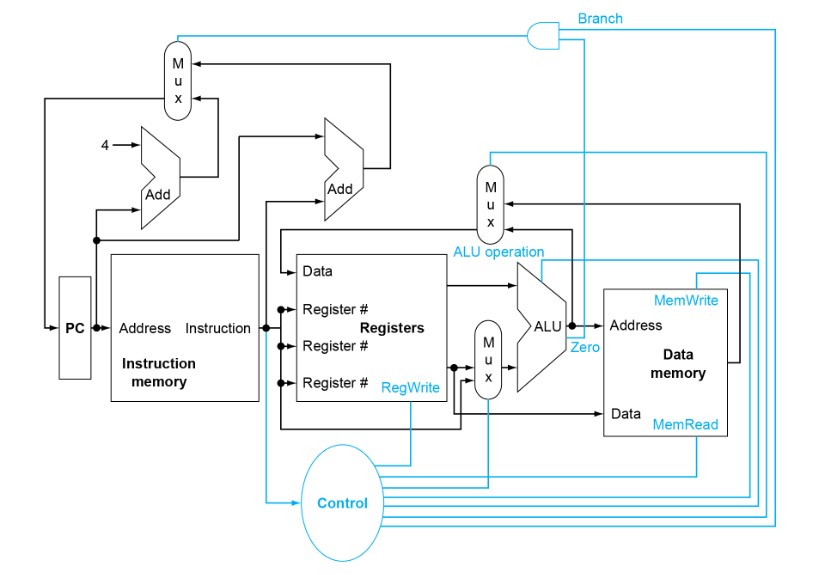
\includegraphics[width = 0.8
        \textwidth]{figures/riscv/risc_2.jpg}
            \caption{\label{risc_2_std} RISC-V Diagram}
        \end{figure}
                    
        
        A processor diagram of the RISC-V CPU can be seen in Figure \ref{risc_2_std}. In the diagram, ``PC'' is the program counter, a 32-bit or 64-bit register; os ``Add'' is an adder; ``Instruction memory'' refers to the component of the processor that stores and supplies the instructions to be executed by the processor; ``Registers'' are small storage units inside the processor that store data and instructions during program execution; ``ALU'' is the arithmetic logic unit; and ``data memory'' is the part of the processor that stores and retrieves data during program execution.
        
        The diagram shows the control unit and its connections in blue. The control unit determines which components should be activated or deactivated, such as the ALU, registers, and multiplexers (MUX), to perform the operations specified by the instructions. The sign in ``RegWrite'' is used to indicate whether the result of an instruction should be rewritten to a register; ``MemRead'' and ``MemWrite'' to indicate whether a memory read or write operation should be performed; ``Branch'' used for implementing conditional branching or jump operations. In control, the ``ALUOperation'' signal can have different values, each corresponding to a specific operation that the ALU should perform. Some common examples of operations controlled by ``ALUOp'' include addition, subtraction, logical operations (AND, OR, XOR), bit shifting, and comparisons. Finally, the ``Zero'' control signal refers to a flag or signal that indicates whether the result of an operation performed by the ALU is equal to zero. This flag is used to make conditional decisions based on the result of a previous operation.
    
    \section{Microcontroller} \label{sec:section_riscv_stud.2}
    
        A microcontroller is a chip that combines a microprocessor with memory, input/output peripherals, and other components needed to perform specific control tasks in an embedded system. It is designed for specific applications that require control, such as embedded systems, industrial automation, consumer electronics devices and more. The microcontroller has integrated resources, such as I/O ports (input/output), analog-digital converters, timers, serial communication and other peripherals that facilitate interaction with the external environment.
        
        In the following section, a microcontroller project using the RISC-V architecture is presented.
        
    
    
    \section{NEORV32 Project} \label{sec:section_riscv_stud.3}
    
        \begin{figure}[!t]
            \begin{center}
                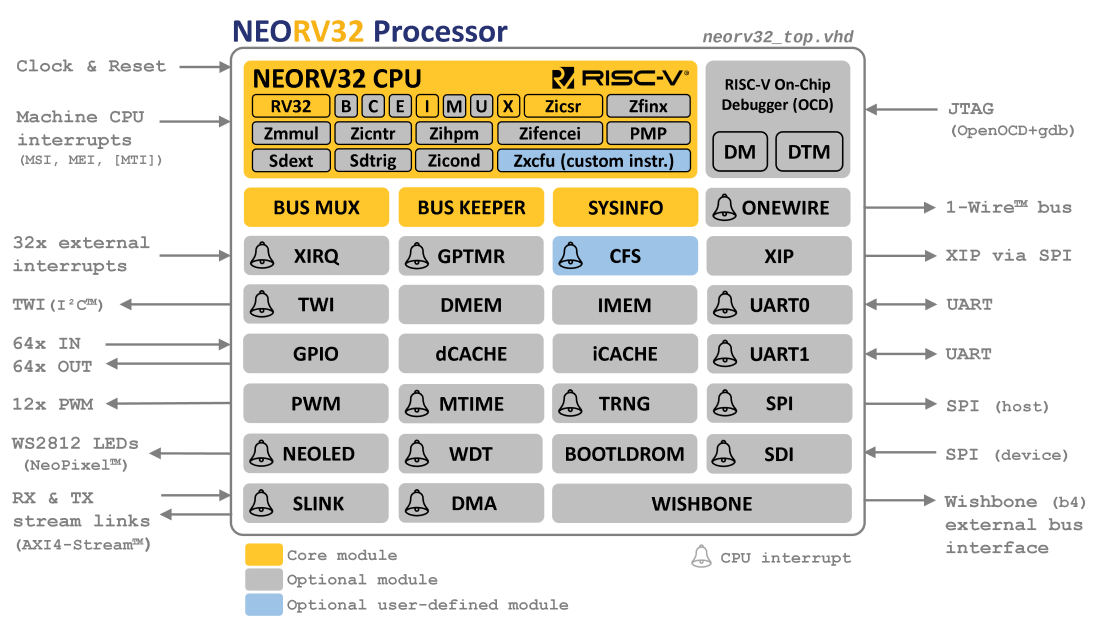
\includegraphics[width=1\textwidth]{figures/neorv32_processor.png}
                \caption{\label{fig:neorv32_peripherals} Representation of the NEORV32 processor, with the available peripherals \cite{nolting_2022}.}
            \end{center}
        \end{figure}
    
        The NEORV32 Project is an open-source, customizable RISC-V processor implementation. It aims to provide a flexible and efficient processor core that can be easily integrated into the FPGA (Field-Programmable Gate Array).
        
        The NEORV32 offers a flexible architecture that allows the connection of multiple peripherals through standard interfaces such as SPI (Serial Peripheral Interface), I2C (Inter-Integrated Circuit), UART (Universal Asynchronous Receiver-Transmitter), GPIO (General Purpose Input/Output). Figure \ref{fig:neorv32_peripherals} shows a diagram of the NEORV32 processor and the components that come with it.
        
        Additionally, the NEORV32 also provides support for external memory, enabling the integration of memory controllers for accessing external storage devices such as flash memory, RAM, SD cards, and others.
        
        The specific peripherals that can be integrated with the NEORV32 depend on the requirements of the project in which it is being used. Some common examples of peripherals that can be added to the NEORV32 include display controllers, audio controllers, network controllers, sensor controllers, wireless communication interfaces, among others.